Given that many of the techniques presented in the dissertation were based on the concepts based on Aitchison geometry, we will provide a brief overview behind Aitchison geometry.\\[5 mm]
%
Aitchison geometry is a framework focused on the analysis of quantities including proportions, percentages, probabilities and concentrations.  These quantities are also referred to as compositions.  At the heart of the framework is the characterization of the Aitchison simplex, where each element of the space is a composition.  A composition can be thought of as a set of proportions, or percentages.\\[5 mm]
%
Linear operations can be defined on compositions, known as ``perturbation'' and ``powering operations''.  These operations are linear in the Aitchison simplex and can be transformed into traditional addition and multiplication operations in Euclidean space through the use of log-ratio transformations.  Inner products can be defined in the Aitchison simplex, giving rise to the distance metrics such as the Aitchison distance.  It can also be shown that the Aitchison simplex forms a finite Hilbert space \cite{Pawlowsky-Glahn2015-qb}. \\[5 mm]
%
\section{Definition}
The Aitchison simplex is formally defined for D species as follows
\[\mathcal{S}^D=\left\{\mathbf{x}=[x_1,x_2,\dots,x_D]\in\mathbb{R}^D \,\left|\, x_i>0,i=1,2,\dots,D; \sum_{i=1}^D x_i=\lambda \right. \right\}. \]
Where $\lambda>0$ can be any positive real-valued constant.  By definition, the compositions are the quantities denoted by $\mathbf{x}$.

 \begin{figure}[H]
         \centering
         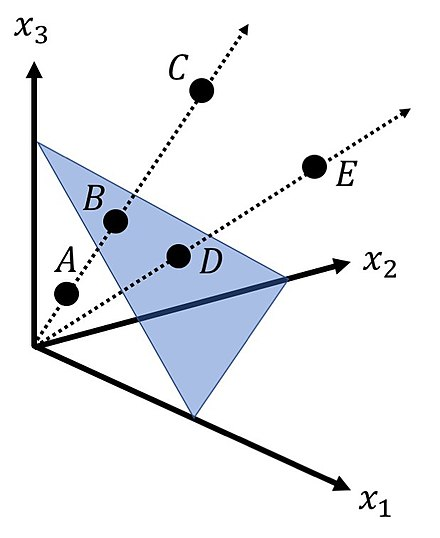
\includegraphics[width=0.5\textwidth]{appendix_c/Aitchison-simplex.jpg}
         \caption[An illustration of the Aitchison simplex.]
                 {An illustration of the Aitchison simplex.  Here, there are 3 parts, $x_1, x_2,  x_3$ represent values of different proportions.  A, B, C, D and E are 5 different compositions within the simplex.  A, B and C are all equivalent and D and E are equivalent.}
         \label{figcS1}
 \end{figure}
There are three core axioms that the Aitchison simplex, namely

\subsection{Scale invariance}
Whether data is represented as proportions, percentages or probabilities, in the context of the Aitchison simplex all of these measurements are equivalent since they only differ by a constant scaling factor.

\subsection{Subcompositional coherence}
Observations on shared species should be consistent. For example, supposed that there are 2 biologists that visited the exact same rainforest to count insects.  One biologist observed 3 species of spiders and 10 species of ants whereas the other biologist only observed 2 species of spiders and 7 species of ants.  If these biologists observed the same 2 spider species and the same 7 species of ants, their conclusions about those species should be the same.  For instance, they should notice that the ratio of those two spider species are consistent between their observations.  While the universal formal definition is still not clearly established, this concept can be formalized to distance metrics as follows

  \[
d(x_k, y_k) \leq d(x, y) \qquad
\forall x, y \in S^D, \; x_k, y_k \in S^k, \; S^k \subset S^D
\]

\subsection{Permutation invariance}
The ordering of how the proportions or were measured or counted doesn't matter.  This is analogous to how combinations are invariant to the order of selection.


\section{Vector Space Structure}
\subsection{Properties}
The Aitchison simplex has the following operators defined using the \textbf{closure} operation as follows

\subsubsection{Perturbation}
\[ x \oplus y = [\frac{x_1 y_1}{\sum_{i=1}^D x_i y_i},\frac{x_2}{\sum_{i=1}^D x_i y_i}, \dots,\frac{x_D y_D}{\sum_{i=1}^D x_i y_i}] =
C[x_1 y_1, ..., x_D y_D]  \qquad \forall x, y \in S^D
\]

\subsubsection{Powering}

\[
\alpha \odot x = [\frac{x_1^{\alpha}}{\sum_{i=1}^D x_i^{\alpha}},\frac{x_2^{\alpha}}{\sum_{i=1}^D x_i^{\alpha}}, \dots,\frac{x_D^{\alpha}}{\sum_{i=1}^D x_i^{\alpha}}] =
C[x_1 y_1, ..., x_D y_D]  \qquad \forall x \in S^D, \quad \alpha \in \mathbb{R}
\]

\subsubsection{Inner product}

\[
\langle x, y \rangle = \frac{1}{2D}
\sum\limits_{i=1}^{D}
\sum\limits_{j=1}^{D}
\log \frac{x_i}{x_j}
\log \frac{y_i}{y_j}
\qquad \forall x, y \in S^D
\]

Under these these operations alone, it is sufficient to show that the Aitchison simplex forms a Euclidean vector space.

\subsection{Orthonormal bases}
Since the Aitchison simplex forms a finite Hilbert space, it is possible to construct orthonormal bases in the simplex. Every composition can be decomposed as follows

\[ x = \bigoplus_{i=1}^D x_i \odot e_i \]

Where $e_1, \ldots e_{D-1} $ forms an orthonormal basis in the simplex \cite{ilr}.

\section{Linear transformations}

There are 3 well-characterized isomorphisms that transform from the Aitchison simplex to real space.  All of these transforms satisfy linearity and as given below

\subsection{Additive Logratio Transform}
The additive log ratio (alr) transform is an where $alr: S^D \rightarrow \mathbb{R}^{D-1} $.  This is given by

\[ alr(x) = \big[ \log \frac{x_1}{x_D} \ldots \log \frac{x_{D-1}}{x_D} \big]\]

The choice of denominator component is arbituary, and could be any specified component.
This transform is commonly used in chemistry with measurements such as pH.  In addition, this is the transform most commonly used for Multinomial logistic regression.  The alr transform is not an isometry, meaning that distances on transformed values will not be equivalent to distances on the original compositions in the simplex.

\subsection{Center Logratio Transform}
The center log ratio (clr) tranform is both an isomorphism and an isometry where \\$clr: S^D \rightarrow \mathbb{U}, \quad U \subset \mathbb{R}^{D} $

\[clr(x) = \big[ \log \frac{x_1}{g(x)} \ldots \log \frac{x_{D-1}}{g(x)} \big] \]

The inverse of this function is also known as the softmax function commonly used in neural networks.

\subsection{Isometric Logratio Transform}
The isometric log ratio (ilr) tranform is both an isomorphism and an isometry where $ilr: S^D \rightarrow \mathbb{R}^{D-1} $

\[
ilr(x) = \big[ \langle x, e_1 \rangle, \ldots \langle x, e_{D-1} \rangle]
\]

There are multiple ways to construct orthonormal bases, including using the Gram–Schmidt process Singular-value decomposition of clr transformed data.
Another alternative is to construct log contrasts from a bifurcating tree.  If are given a bifurcating tree, we can construct a basis from the internal nodes in the tree.

 \begin{figure}[H]
         \centering
         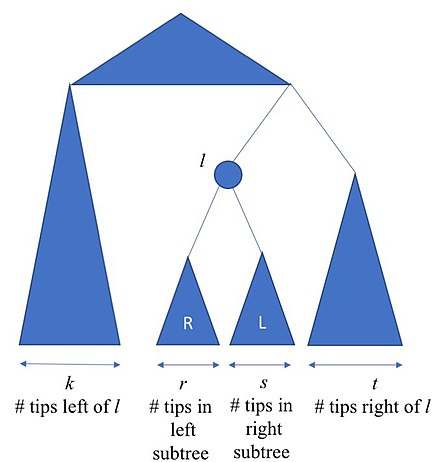
\includegraphics[width=0.5\textwidth]{appendix_c/Orthogonal-tree-basis.jpg}
         \caption[An illustration of the bifurcating trees as an orthonormal basis.]
                 {A representation of a tree in terms of its orthogonal components. l represents an internal node, an element of the orthonormal basis. This is a precursor to using the tree as a scaffold for the ilr transform.}
         \label{figcS1}
 \end{figure}

Each vector in the basis would be determined as follows

\[e_l = C[exp( \underbrace{0,...0}_{k}, \underbrace{a,...,a}_{r},\underbrace{b,...,b}_s,\underbrace{0,...0)}_t]\]

The elements within each vector are given as follows

\[a = \frac{\sqrt{s}}{\sqrt{r(r+s)}} \quad \textrm{and} \quad b = \frac{-\sqrt{r}}{\sqrt{s(r+s)}}\]

where $k, r, s, t$ are the respective number of tips in the corresponding subtrees shown in the figure.  It can be shown that the resulting basis is orthonormal \cite{groups_of_parts}.

Once the basis $\Psi$ is built, the ilr transform can be calculated as follows

\[
ilr(x) = C[\exp(clr(x) \Psi)]
\]


where each element in the ilr transformed data is of the following form


\[
b_i = \sqrt{\frac{rs}{r+s}} \log \frac{g(x_R)}{g(x_S)}
\]

where $ x_R$ and $ x_S$ are the set of values corresponding to the tips in the subtrees $R$ and $S$.
